\documentclass[a4paper]{article}
\usepackage{ulem}
\usepackage{graphicx}
\usepackage[namelimits]{amsmath}
\usepackage{amssymb}
\usepackage{amsmath}
\usepackage{amsfonts}
\usepackage{mathrsfs}
\usepackage{enumerate}
\usepackage{indentfirst}
\usepackage{multirow}
\usepackage{latexsym}
\usepackage{subfig}
\usepackage{listings}
\usepackage{xcolor}
\usepackage{algorithm}
\usepackage{algpseudocode}
\usepackage{caption}

\lstset{numbers=left,
	numberstyle=\tiny,
	frame=shadowbox,
	backgroundcolor=\color[RGB]{245,245,244},
	keywordstyle=\color[RGB]{40,40,255},
	numberstyle=\footnotesize\color{darkgray},
	commentstyle=\color[RGB]{50,50,50},
	breaklines=true}

\renewcommand{\algorithmicrequire}{\textbf{Input:}}
\renewcommand{\algorithmicensure}{\textbf{Output:}}

\title{UM-SJTU JOINT INSTITUTE\\VE475 Introduction to Cryptography\\\vspace{0.5cm} Homework 2}
\author{Li Yong 517370910222}
\begin{document}
\maketitle
\newpage

\section*{Ex.1 Simple questions}
	\begin{enumerate}
		\item
		$$17 \cdot 6 \equiv 1 \bmod 101$$
		\item
		$$gcd(12, 236) = 4 \Rightarrow 3x \equiv 7 \bmod 59$$
		$$x \equiv 22 \bmod 59$$
		$$x \equiv (22 + 59k) \bmod 236, k \in \{0, 1, 2, 3\}$$
		\item
		We calculate the corresponding ciphertext $c$ for given plaintext $m$.
		\begin{table}[htbp]
  		\centering
	    \begin{tabular}{c|cccccccccccccccc}
			\hline
	    m     & 0     & 1     & 2     & 3     & 4     & 5     & 6     & 7     & 8     & 9     & 10    & 11    & 12    & 13    & 14    & 15 \\
			\hline
	    c     & 0     & 1     & 4     & 17    & 16    & 5     & 6     & 28    & 2     & 10    & 20    & 13    & 24    & 22    & 19    & 23 \\
			\hline
	    m     & 16    & 17    & 18    & 19    & 20    & 21    & 22    & 23    & 24    & 25    & 26    & 27    & 28    & 29    & 30    &  \\
			\hline
	    c     & 8     & 12    & 9     & 7     & 18    & 11    & 21    & 29    & 3     & 25    & 26    & 15    & 14    & 27    & 30    &  \\
			\hline
    	\end{tabular}
		\end{table}
		\par Plot the table, it is obviously a bijection. Hence we can decrypt the message by this table.
		\begin{figure}[!htb]
			\centering
			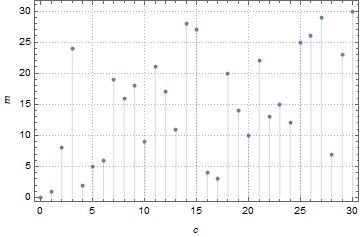
\includegraphics[scale=0.7]{1.png}
		\end{figure}
		\item
		$$4883 = 19 \times 257$$
		$$4369 = 17 \times 257$$
		\item
		$$
		A = \left(
		\begin{matrix}
			3 & 5 \\
			7 & 3 \\
		\end{matrix}
		\right)\\
		$$
		$$\det{A} = -26$$
		Suppose $A$ is invertible modulo $p$, then
		$$\det{(A)} \cdot t \equiv 1 \bmod p$$
		$$26t \equiv 1 \bmod p$$
		So that $26$ and $p$ are coprime. Hence when $p = 2$, $A$ is not invertible.
		\item
		$$ab \equiv 0 \bmod p$$
		$$\Rightarrow p \mid ab$$
		$p$ is prime so that gcd$(a, p) = 1$ or gcd$(a, p) = p$.
		\begin{enumerate}[a.]
			\item If gcd$(a, p) = 1$, then $p \mid n, \ i.e.,\ b$ is congruent to $0 \bmod p \footnote{According to hw1 Ex. 1.3}$.
			\item If gcd$(a, p) = p$, then $a$ is congruent to $0 \bmod p$.
		\end{enumerate}
		\item
		 $$
		 \begin{aligned}
			 2^{2017} \bmod 5 &= 2 \cdot 4^{1008} \bmod 5\\
			 &= 2 \cdot (-1)^{1008} \bmod 5\\
			 &= 2 \bmod 5 = 2
	 	 \end{aligned}
		 $$
		 $$
		 \begin{aligned}
			 2^{2017} \bmod 13 &= 2 \cdot 64^{336} \bmod 13\\
			 &= 2 \cdot (-1)^{336} \bmod 13\\
			 &= 2 \bmod 13 = 2
	 	 \end{aligned}
		 $$
		 $$
		 \begin{aligned}
			 2^{2017} \bmod 31 &= 4 \cdot 32^{403} \bmod 31\\
			 &= 4 \cdot (-1)^{403} \bmod 31\\
			 &= 4 \bmod 31 = 4
	 	 \end{aligned}
		 $$
		 According to CRT,
		 $$
		 \left\{
		 \begin{aligned}
			 &2^{2017} \equiv 2 \bmod 5\\
			 &2^{2017} \equiv 2 \bmod 13\\
			 &2^{2017} \equiv 4 \bmod 31\\
		 \end{aligned}
		 \right.
		 $$
		 So that
		 $$2^{2017} \bmod 2015 = 2 \times M_{1}t_{1} + 2 \times M_{2}t_{2} + 4 \times M_{3}t_{3}\ (\bmod\ 2015),$$
		 where
		 $$
		 \begin{aligned}
			 M_{1} &= 13 \times 31\\
			 M_{2} &= 5 \times 31\\
			 M_{3} &= 5 \times 13\\
		 \end{aligned}
		 $$
		 $$
		 \left\{
		 \begin{aligned}
			 &(M_{1}t_{1}) \equiv 1 \bmod 5\\
			 &(M_{2}t_{2}) \equiv 1 \bmod 13\\
			 &(M_{3}t_{3}) \equiv 1 \bmod 31\\
		 \end{aligned}
		 \right.
		 $$
		 Hence, $2^{2017} \equiv 717 \bmod 2015$.
	\end{enumerate}

\section*{Ex.2 Rabin cryptosystem}
	\begin{enumerate}
		\item {\bf Rabin cryptosystem} is an asymmetric cryptographic technique. As with all asymmetric cryptosystems, the Rabin system uses both a public and a private key.
		\par The keys are generated in such process:
		\begin{enumerate}[$\bullet$]
			\item Choose two large distinct primes $p$ and $q$ as private keys.
			\item Then public key is $n = pq$.
		\end{enumerate}
		\par For the encryption, only public key is needed, while for the decryption, private key is used.
		\par Given a plaintext $m$ modulo $n$, its corresponding ciphertext is $c = m^{2} \bmod 3n$.
		\item
		\begin{enumerate}[a)]
			\item According to the computation of square roots modulo introduced in Rabin cryptosystem, there are on ly four possible results. Hence, a meaningful message can be expected fairly soon.
			\item No. For decryption, she needs two private keys to calculate the square roots modulo. Even if she could factor public key to get private keys, $p$ and $q$ are large primes. So that it would take Eve much time to decrypt.
			\item CCA.
			\par Given ciphertext $c$, she could use this device to get 4 result. We denote them as $+r$, $-r$, $+s$ and $-s$. Then
			$$gcd((+r) - (+s), n) = q$$
			$$gcd((+r) - (-s), n) = p$$
		\end{enumerate}
	\end{enumerate}

\section*{Ex.3 CRT}
	$$
	\left\{
	\begin{aligned}
		&x \equiv 1 \bmod 3\\
		&x \equiv 2 \bmod 4\\
		&x \equiv 3 \bmod 5\\
	\end{aligned}
	\right.
	$$
	So that
	$$x \bmod 60 = 1 \times M_{1}t_{1} + 2 \times M_{2}t_{2} + 3 \times M_{3}t_{3}\ (\bmod\ 60),$$
	where
	$$
	\begin{aligned}
		M_{1} &= 4 \times 5\\
		M_{2} &= 3 \times 5\\
		M_{3} &= 3 \times 4\\
	\end{aligned}
	$$
	$$
	\left\{
	\begin{aligned}
		&(M_{1}t_{1}) \equiv 1 \bmod 3\\
		&(M_{2}t_{2}) \equiv 1 \bmod 4\\
		&(M_{3}t_{3}) \equiv 1 \bmod 5\\
	\end{aligned}
	\right.
	$$
	Hence, $x \equiv 58 \bmod 60$. The two smallest possible numbers of people in the group are $58$ and $118$.

\section*{References}
\begin{enumerate}
	\item https://cryptography.fandom.com/wiki/Rabin\_cryptosystem
\end{enumerate}
\end{document}
